% !TeX program = xelatex
% !TeX encoding = UTF-8
% !TeX spellcheck = en_US
% !BIB program = biber
% !TEX root = ./main.tex 
%% 
%% The above lines help editors like TeXstudio to automatically choose the right tools
%% to compile your LaTeX source file. If your tool does not support these magic comments,
%% You will need to make appropriate manual choices.
%% 
%% You can safely use "pdflatex" instead of "xelatex" if you prefer the pdfLaTeX toolchain.
%% However, pdfLaTeX will not be able to deliver the professional font experience that you
%% will get with XeLaTeX.
%% 
%% _Important_: These magic comments should be on the first lines of your source file.
%% 
%%%%%%%%%%%%%%%%%%%%%%%%%%%%%%%%%%%%%%%%%%%%%%%%%%%%%%%%%%%%%%%%%%%%%%%%%%%%%%%%

%%%%%%%%%%%%%%%%%%%%%%%%%%%%%%%%%%%%%%%%%%%%%%%%%%%%%%%%%%%%%%%%%%%%%%%%%%%%%%%%
%% 
%%            JJJJ   K                         K   UUUU         UUUU  
%%            JJJJ   KKKK                   KKKK   UUUU         UUUU  
%%            JJJJ   KKKKKK               KKKKKK   UUUU         UUUU  
%%            JJJJ      KKKKKK         KKKKKK      UUUU         UUUU  
%%            JJJJ         KKKKKK   KKKKKK         UUUU         UUUU  
%%            JJJJ            KKKKKKKKK            UUUU         UUUU  
%%    JJ     JJJJJ               KKK               UUUUU       UUUUU  
%%  JJJJJJJJJJJJJ    KKKKKKKKKKKKKKKKKKKKKKKKKKK    UUUUUUUUUUUUUUU   
%%    JJJJJJJJJ      KKKKKKKKKKKKKKKKKKKKKKKKKKK      UUUUUUUUUUU     
%% 
%% This is an example file for using the JKU LaTeX Beamer Theme.
%% 
%% Template created by Susanne Hametner and Doris Pargfrieder
%% Template altered by Pieter-Jan Hoedt (2020)
%% Template rewritten by Michael Roland (2021)
%% 
%%%%%%%%%%%%%%%%%%%%%%%%%%%%%%%%%%%%%%%%%%%%%%%%%%%%%%%%%%%%%%%%%%%%%%%%%%%%%%%%

%%%%%%%%%%%%%%%%%%%%%%%%%%%%%%%%%%%%%%%%%%%%%%%%%%%%%%%%%%%%%%%%%%%%%%%%%%%%%%%%
%% 
%% Document class: This is a LaTeX beamer presentation.
%% 
\documentclass[utf8,aspectratio=1610,ngerman,english]{beamer}
%% 
%% The comma-separated list in square brackets are class options.
%% Useful options that you might want to use:
%% 
%% Define the aspect ratio of the slide layout:
%%  * aspectratio=169  ... 16:9 aspect ratio
%%  * aspectratio=43   ... 4:3 aspect ratio
%%  * aspectratio=1610 ... 16:10 aspect ratio
%% 
%% Define document languages:
%%  * ngerman ... German
%%  * english ... English
%%  * ...
%% 
%% Note that adding multiple document languages allows you to switch between these languages
%% within the document (using e.g. the `otherlanguage' environment). The last language in
%% the class options will be used as the default document language.
%% 
%% Switch to handout mode:
%%  * handout ... A compact mode that allows you to remove animation and skips slides for
%%                efficient printing.
%% 
%% Other options:
%%  * utf8 ... Treat input files as UTF-8 encoded. Make sure to always provide that option
%%             when you use pdfLaTeX so that pdfLaTeX knows how to read and interpret
%%             characters this source file.
%%  * c    ... Vertically center text on slides by default. You should avoid using this
%%             option. Only use this to restore the behavior of older versions of this theme.
%% 
%% _Important_: The document class should be the first line of LaTeX code in your main
%% source file. Do not place anything but comments / magic comments above that line (unless
%% you really know what you are doing).
%% 
%%%%%%%%%%%%%%%%%%%%%%%%%%%%%%%%%%%%%%%%%%%%%%%%%%%%%%%%%%%%%%%%%%%%%%%%%%%%%%%%

%%%%%%%%%%%%%%%%%%%%%%%%%%%%%%%%%%%%%%%%%%%%%%%%%%%%%%%%%%%%%%%%%%%%%%%%%%%%%%%%
%% 
%% Use the JKU LaTeX beamer theme for this presentation.
%% 
%\usetheme[TNF,nosectionpage]{jku}
\usetheme[darkmode,fancyfonts,framenumber,mathastext, SOWI]{jku}
%% 
%% The comma-separated list in square brackets are theme options. Useful options that you
%% might want to use:
%% 
%% Color scheme selection options:
%%  * JKU  ... Use JKU (gray) color scheme (this is the default if no scheme is selected).
%%  * BUS  ... Use Business School color scheme.
%%  * LIT  ... Use Linz Institute of Technology color scheme.
%%  * MED  ... Use MED faculty color scheme.
%%  * RE   ... Use RE faculty color scheme.
%%  * SOE  ... Use School of Education color scheme.
%%  * SOWI ... Use SOWI faculty color scheme.
%%  * TNF  ... Use TNF faculty color scheme.
%% 
%% Color mode selection options:
%%  * darkmode ... Use dark color mode (where title and logo frames have a dark background).
%% 
%% Frame numbering options:
%%  * framenumber         ... Insert frame number into the frame footer.
%%  * totalframenumber    ... Insert frame number and total frame number into the frame footer
%%                            (only frames in the main part are counted).
%%  * appendixframenumber ... Similar to `totalframenumber', but count the overall total frame
%%                            number of main part and appendix.
%% 
%% Note that combining `totalframenumber' and `appendixframenumber' options will show the total
%% number of frames for the main part on frames in the main part and the overal total number of
%% frames for frames in the appendix.
%% 
%% Sectioning options:
%%  * nosectionpage       ... Supress section frames (see \section{<title>} command).
%%  * nosubsectionpage    ... Supress subsection frames (see \subsection{<title>} command).
%%  * nosubsubsectionpage ... Supress subsubsection frames (see \subsubsection{<title>} command).
%%  * partpage            ... Insert part frames (see \part{<title>} command).
%% 
%% Note that `nosectionpage' automatically sets `nosubsectionpage' and `nosubsubsectionpage'.
%% You could still e.g. show only subsubsection pages by using `nosectionpage,subsubsectionpage'.
%% 
%% Space-efficient monospace font options (requires XeTeX):
%%  * compactmono   ... Use condensed fixed-width font everywhere.
%%  * nocompactverb ... Do not use condensed fixed-width font for verbatim and listings.
%% 
%% Style-breaking options:
%%  * nojkufooter    ... Do not insert JKU/partner logos into the frame footer.
%%  * nofooter       ... Do not display a frame footer.
%%  * noimprint      ... Do not insert imprint on title pages.
%%  * nojkulogo      ... Do not insert JKU & K logos on title pages and in frame footers.
%%  * frametitlecaps ... Set frame titles in capital letters (like in eariler theme versions).
%%  * nofancyfonts   ... Do not use custom TTF fonts with XeTeX / supress pdfLaTeX warning.
%%  * mac            ... Use adapted color palette for screen display on Mac.
%%  * legacyitemizestyle ... Use old bullet style in itemization.
%% 
%% Experimental options:
%%  * mathastext ... Use standard document fonts (and default to sans-serif font) in math mode
%% 
%% Advanced options:
%%  * nooptpackages     ... Do not load additional convenience packages (which are only there
%%                          to provide interoperability to the behavior of previous versions of
%%                          this theme but are not actually required for the current version).
%%  * logopath={<path>} ... Set the path where the theme can find its own logo resources. This
%%                          should typically be a relative path and the default is `./logos'.
%%  * fontpath={<path>} ... Set the path where the theme can find its own font resources. This
%%                          should typically be a relative path and the default is `./fonts'.
%% 
%% Hint: Boolean options can be used in the forms `option' or `option=true' the enable the
%% option and `nooption' or `option=false' to disable the option.
%% 
%%%%%%%%%%%%%%%%%%%%%%%%%%%%%%%%%%%%%%%%%%%%%%%%%%%%%%%%%%%%%%%%%%%%%%%%%%%%%%%%

%%%%%%%%%%%%%%%%%%%%%%%%%%%%%%%%%%%%%%%%%%%%%%%%%%%%%%%%%%%%%%%%%%%%%%%%%%%%%%%%
%% 
%% This is the place where you can load additional packages. If you want to load
%% a package `booktabs', you would use the command `\usepackage{booktabs}'.
%% 

\usepackage{booktabs}
\usepackage{tabularx}
%\usepackage{pifont}
%\newcommand{\cmark}{\ding{51}}
%\newcommand{\xmark}{\ding{55}}
%\newcommand{\rarr}{\ding{212}}
%\newcommand{\larr}{\raisebox{\depth}{\rotatebox{180}{\rarr}}}
\usepackage{csquotes}
\usepackage[%
    backend=biber,
    citestyle=authoryear,
    sortcites=true, 
    firstinits=true,
    sortcites=true,
    maxbibnames=10,
    natbib
]{biblatex}
\usepackage{animate}
\usepackage[caption=false]{subfig}
\usepackage{xspace}

\renewcommand{\emph}[1]{\textcolor{jkuGreen}{#1}}
% \newcommand{\nPC}{\hyperref[eq:nPC]{\texttt{(nPC1)}}}
% \newcommand{\nPCY}{\hyperref[eq:nPCY]{\texttt{(nPC2)}}}
% \newcommand{\nPCE}{\hyperref[eq:nPCE]{\texttt{(nPC3)}}}
% \newcommand{\npCP}{\emph{(npCP)}}
% \newcommand{\pCP}{\emph{(pCP)}}
\def\Cplusplus{C\raisebox{0.5ex}{\tiny\textbf{++}}}

\newtheorem{observation}{Observation}
\newtheorem{proposition}{Proposition}
\newcommand{\nPC}{\hyperref[eq:nPC]{\texttt{(nPC1)}}\xspace}
\newcommand{\nPCE}{\hyperref[eq:nPCE]{\texttt{(nPC3)}}\xspace}
\newcommand{\nPCY}{\hyperref[eq:nPCY]{\texttt{(nPC2)}}\xspace}
\newcommand{\nPCYR}{\hyperref[eq:nPCYR]{\texttt{(nPCR)}}\xspace}
\newcommand{\nPCYRN}{\hyperref[eq:nPCYRN]{\texttt{(nPCR2)}}\xspace}
\newcommand{\tsplib}{\texttt{TSPlib}\xspace}
\newcommand{\pmed}{\texttt{pmed}\xspace}
\newcommand{\pCP}{($p$CP)\xspace}
\newcommand{\npCP}{(n-$p$CP)\xspace}
\newcommand{\PC}{\hyperref[eq:PC]{\texttt{(PC1)}}\xspace}
\newcommand{\PCE}{\hyperref[eq:PCE]{\texttt{(PC3)}}\xspace}
\newcommand{\PCY}{\hyperref[eq:PCY]{\texttt{(PC2)}}\xspace}
\newcommand{\inI}{i \in \mathcal I}
\newcommand{\inJ}{j \in \mathcal J}
\newcommand{\inH}{h \in \mathcal H}
\newcommand{\noPP}{\texttt{B}\xspace}
\newcommand{\PP}{\texttt{P}\xspace}
\newcommand{\sH}{\texttt{PH}\xspace}
\newcommand{\prio}{\texttt{PHB}\xspace}

%% 
%%%%%%%%%%%%%%%%%%%%%%%%%%%%%%%%%%%%%%%%%%%%%%%%%%%%%%%%%%%%%%%%%%%%%%%%%%%%%%%%

%%%%%%%%%%%%%%%%%%%%%%%%%%%%%%%%%%%%%%%%%%%%%%%%%%%%%%%%%%%%%%%%%%%%%%%%%%%%%%%%
%% 
%% Set reasonable defaults for biblatex.
%% 

\preto{\bibsetup}{\providecommand*{\insertbiblabel}{}}
\DeclareFieldFormat*{title}{#1}
\DeclareFieldFormat*{booktitle}{#1}
\DeclareFieldFormat*{journaltitle}{#1}
\setcounter{biburlnumpenalty}{100}
\setcounter{biburllcpenalty}{100}
\setcounter{biburlucpenalty}{100}

%% Add bibligraphy source files
\addbibresource{references.bib}


\setbeamertemplate{theorems}[numbered]
\setbeamertemplate{definitions}[numbered]
\setbeamertemplate{lemmas}[numbered]

%\setbeamerfont{block title}{}

\setbeamercolor{block title}{bg=jkuGreen,fg=white}

\graphicspath{{../../Master Thesis/final_plots/}}

%% 
%%%%%%%%%%%%%%%%%%%%%%%%%%%%%%%%%%%%%%%%%%%%%%%%%%%%%%%%%%%%%%%%%%%%%%%%%%%%%%%%

\begin{document}

%%%%%%%%%%%%%%%%%%%%%%%%%%%%%%%%%%%%%%%%%%%%%%%%%%%%%%%%%%%%%%%%%%%%%%%%%%%%%%%%
%% 
%% Presentation information and title page
%% 

%% Command \series{series title}: sets the series title
%\series{Space for your lecure title}

%% Command \title[short title]{title}: sets the presentation title
%% Command \titlesmall{text}: switches to small font size inside title
\title{On the nested $p$-center problem}

%% Command \subtitle[short subtitle]{subtitle}: sets the presentation subtitle
%\subtitle{Master Thesis Seminar}
%\subtitle{Christof Brandstetter, BSc}


%% Command \author[short authors]{authors}: sets the presentation authors (multiple authors may be separated with \and)
%\author{Christof Brandstetter \and Supervisor: Univ.-Prof. DI Markus Sinnl, BSc PhD}
\author{\underline{Christof Brandstetter} \and Markus Sinnl}

%% Command \institute{name}: sets the institute / author affiliation (style-breaking)
\institute{Institute of Business Analytics and Technology Transformation / JKU Business School, \\Johannes Kepler University Linz \\ This research was funded in whole, or in part, by the Austrian Science Fund (FWF) [P 35160-N]. }

%% Command \institutecode{CODE}: sets the institute abbreviation/initials (used to load the institute logo file, if present)
%\institutecode{INS}

%% Command \date[short date]{date}: sets the presentation date (short date is used in the footer by default)
%\date{\today}  % use this to set the date on the title page (style-breaking) and in the footer
%\date[\today]{} % use this to set the date except for the title page (effectively in the footer only)
\date{\today}

%% Command \partnerlogo[white=filename]{filename}: use filename as partner logo (leave filename blank to disable the partner logo), the optional argument ``white='' defines a separate file for use on dark background
\partnerlogo{logos/inoc.png}

%% Command \footer{text}: sets the footer field
%\footer{\insertshortsectiontitle} % the default
\footer{\insertshorttitle}        % a good alternative

%% Command \footerdate{text}: sets the footer date field
%\footerdate{\insertshortdate} % the default

%% Command \footerpartnerlogo{filename}: use a different partner logo in the footer (e.g. a logo with a different form factor or no filename to disable the partner logo in the footer)
%\footerpartnerlogo{our_partner_logo}

%% Command \agenda[caption]{text}: sets the agenda (and optional caption) to display on the next title or section page
%\agenda[caption]{text}


%% Finally, print the title page using the above information:
%% 
%% \maketitle[options]
%%     Inserts a title page. The current standard faculty color theme and color
%%     mode are used by default, you may modify this using any of the following
%%     options:
%%      * light ... use light color theme
%%      * dark  ... use dark color theme
%%      * gray  ... use JKU gray color theme
%%      * black ... use black background
%%     In addition, options may contain a faculty name (see theme options) to
%%     use the faculty's color theme, e.g. `\maketitle[LIT,dark]'.
%% 
\maketitle
%% 
%% Note that you can even change the presentation information and print another
%% title page (with that updated information) ANYWHERE in your presentation.
%% 
%%%%%%%%%%%%%%%%%%%%%%%%%%%%%%%%%%%%%%%%%%%%%%%%%%%%%%%%%%%%%%%%%%%%%%%%%%%%%%%%


%% 
%% You can split your presentation into sections, subsections, and subsubsections,
%% just like you would do with any other LaTeX document. Depending on the chosen
%% theme options, frames showing the section titles will be inserted for each
%% sectioning command. You can use the starred versions of these commands (e.g.
%% `\section*{<title>}') to suppress specific section title frames.
%% 

% \section*{Introdcution}
% \begin{frame}{Introduction}
%     \begin{itemize}
%         \item \emph{$p$-center problem} \pCP: open $p$ number of facilities, such that the maximum distance between a customer and its closest open facility minimized \pause
%         %\item \emph{nested}: sets of later periods contain more facilities and have to contain the facilities of sets of previous periods \pause
%         \item \emph{nested}: considering more than one time period in which facilities are opened, facilities once open cannot be closed \pause
%         %\item \emph{nested $p$-center problem} \npCP: choose a set of $p^h$ facilities over different time periods h, such that the sum of the maximum distance between a demand point and its closest facility belonging to that set in that time period over all periods is minimized and the sets are nested 
%         \item \emph{nested $p$-center problem} \npCP: open $p^h$ number of \emph{nested} facilities in period $h$, such that the sum of the maximum distances between a customer and its closest open facility in this time period is minimized
%     \end{itemize}
% \end{frame}
\begin{frame}{The $p$-center problem \pCP:}
    \begin{block}{Definition}
        \begin{itemize}\pause
            \item given
                  \begin{itemize}
                      \item a set V of locations, \pause
                      \item \emph{$p$} $\in \mathbb{Z}$, and \pause
                      \item \emph{distances} $\emph{d_{ij}}$ from location $i \in V$ to $j \in V$ \pause
                  \end{itemize}
            \item we want to
                  \begin{itemize}
                      \item \emph{open \textit{p} locations} of V, such that \pause
                      \item the \emph{maximum distance} of any location to its closest opened location is \emph{minimized}.
                  \end{itemize}
        \end{itemize}
    \end{block}
    \citet{Hakimi1964,Elloumi2018,contardo2019scalable,GAAR2022}
\end{frame}
% TODO ask Markus about the definition for nesting, especially about the need of redifining the V and iff
\begin{frame}{The nesting property for location problems}
    \begin{block}{Definition}
        \setbeamerfont{item}{size=\footnotesize}
        \setbeamerfont{subitem}{size=\footnotesize}
        \begin{itemize}
            \item given
                  \begin{itemize}
                      \item a set of locations $V$ \pause
                      \item a set of time periods $\mathcal{H} = \left\{1, \dots, H\right\}$ and \pause
                      \item a set of integers $\mathcal P = \left\{p^1, \dots, p^H\right\}$ indicating the number of facilities to open \pause
                      \item where $p^h \leq p^{h+1}$ for $h = 1, \dots, H-1$ \pause
                  \end{itemize}
            \item the subsets $V^h \subseteq V$ with $|V^h| = p^h$ \pause
            \item are called \emph{nested} iff $V^h  \subseteq V^{h+1}$ for $h = 1, \dots, H-1$
        \end{itemize}
    \end{block}\pause
    Introduced by \citet{Roodman1975} and used in e.g., \citet{albareda2009multi,bakker2024value} and reintroduced as nesting by \citet{McGarvey2022}
\end{frame}

\begin{frame}{$p$-center problem vs nested $p$-center problem}
    \centering
    %    \vspace{-10pt}
    \begin{figure}
        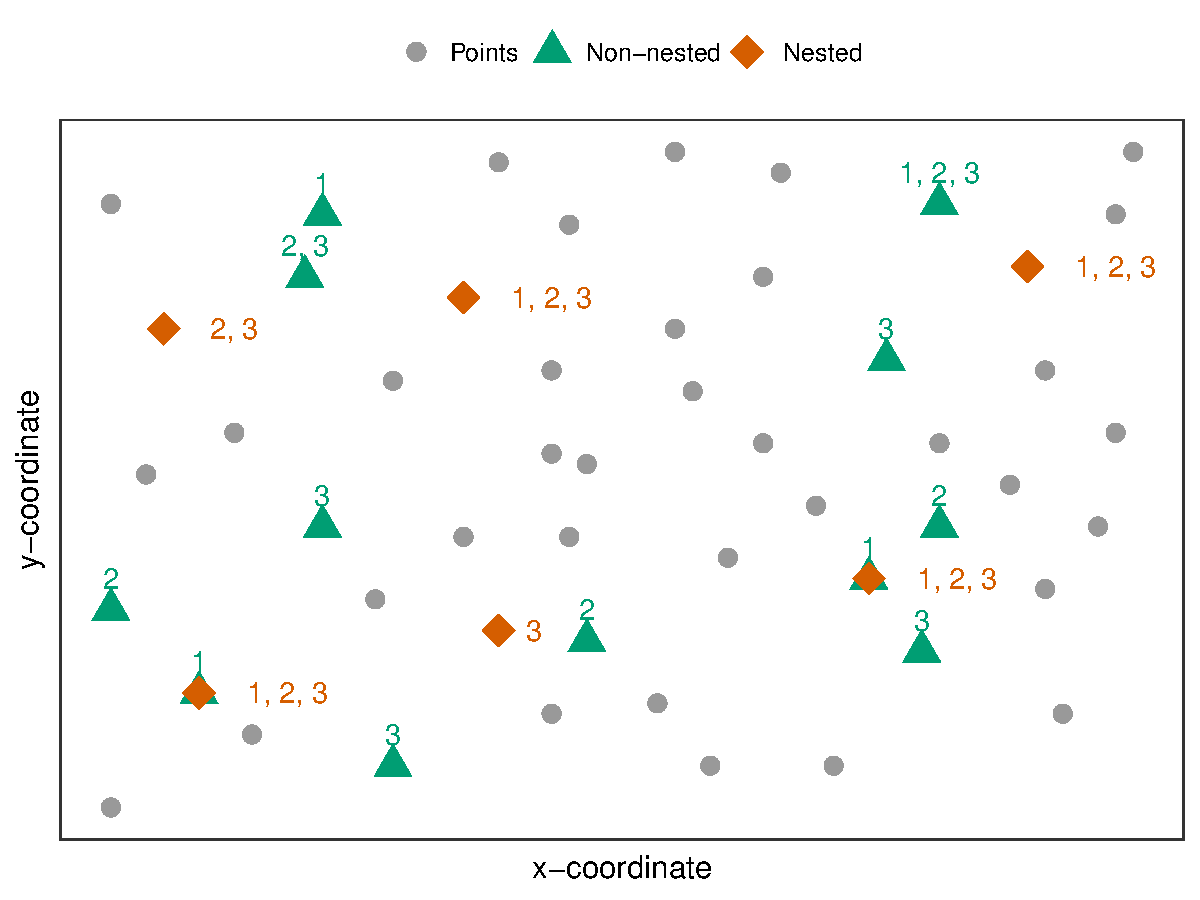
\includegraphics[width=0.55\linewidth]{images/Rplot01.pdf}
        \caption{Optimal solution of \pCP with $p=4,5,6$ and \npCP with $\mathcal P = \{4,5,6\}$}
    \end{figure}
\end{frame}

% \begin{frame}{The nested \textit{p}-center problem: Definition}
%     \setbeamerfont{item}{size=\footnotesize}
%     \setbeamerfont{subitem}{size=\footnotesize}
%     \begin{minipage}{0.48\textwidth}
%         \begin{block}{Definition I}
%             \begin{itemize}
%                 \item given a set of customer demand points $\mathcal I$, \pause
%                 \item potential facility locations $\mathcal J$, \pause
%                 \item time periods $\mathcal H = \left \{1,\dots,H \right \}$, \pause
%                 %\item integers $\mathcal P = \left \{p^1, \dots p^H \right \}$ where $p^h \leq p^{h+1}$ for $h = 1, \dots, H-1$ and $p^H \leq \left\lvert \mathcal J \right\rvert$ 
%                 \item integers $\mathcal P = \left \{p^1, \dots p^H \right \}$   \pause
%                 \begin{itemize} 
%                     \item where $p^h \leq p^{h+1}$ for $h = 1, \dots, H-1$ and
%                     \item $p^H \leq \left\lvert \mathcal J \right\rvert$
%                 \end{itemize} \pause
%                 \item distances $d_{ij} \geq 0$ between each $i \in \mathcal I$ and $j \in \mathcal J$ \pause
%             \end{itemize}
%         \end{block}
%     \end{minipage}
%     \begin{minipage}{0.48\textwidth}
%         \begin{block}{Definition II}
%             \vspace*{3pt}
%             \begin{itemize}
%                 %\item a feasible solution to the nested $p$-center problem consists of a set $\mathcal J^h \subseteq \mathcal J$ with $\left\lvert \mathcal J^h \right\rvert = p^h$ for $h \in \mathcal H$, for which $\mathcal J^h \subseteq \mathcal J^{h+1}$ for $h = 1, \dots, H-1$ holds
%                 \item a feasible solution to the nested $p$-center problem consists of a set $\mathcal J^h \subseteq \mathcal J$ \pause
%                 \begin{itemize}
%                     \item with $\left\lvert \mathcal J^h \right\rvert = p^h$ for $h \in \mathcal H$,
%                     \item for which $\mathcal J^h \subseteq \mathcal J^{h+1}$ for $h = 1, \dots, H-1$ holds \pause
%                     %\item for which $\mathcal J^h \subseteq \mathcal J^{h+1}$ for $h \in \mathcal H \setminus \left \{H \right \}$ holds
%                 \end{itemize} 
%                 %\item the goal is to find a feasible solution which minimizes $\sum_{h = 1}^{H} d_h(\mathcal J^h)$, where $d_h(\mathcal J^h) = \max_{i \in \mathcal I}\min_{j \in \mathcal J^h} d_{ij}$ for $h \in \mathcal H$
%                 \item the goal is to find a feasible solution which minimizes $\sum_{h = 1}^{H} d_h(\mathcal J^h)$, 
%                 \begin{itemize}
%                     \item where $d_h(\mathcal J^h) = \max_{i \in \mathcal I}\min_{j \in \mathcal J^h} d_{ij}$ for $h \in \mathcal H$
%                 \end{itemize}
%             \end{itemize}
%             \vspace*{3pt}
%         \end{block}
%     \end{minipage}
% \end{frame}

\begin{frame}{The nested \textit{p}-center problem}
    \setbeamerfont{item}{size=\footnotesize}
    \setbeamerfont{subitem}{size=\footnotesize}
    \begin{minipage}{0.48\textwidth}
        \begin{block}{Definition part I}
            \vspace*{13pt}
            \begin{itemize}
                \setlength\itemsep{1em}
                \item given a set of locations $V$, \pause
                \item time periods $\mathcal H = \left \{1,\dots,H \right \}$, \pause
                      %\item integers $\mathcal P = \left \{p^1, \dots p^H \right \}$ where $p^h \leq p^{h+1}$ for $h = 1, \dots, H-1$ and $p^H \leq \left\lvert \mathcal J \right\rvert$ 
                \item integers $\mathcal P = \left \{p^1, \dots p^H \right \}$   \pause
                      \begin{itemize}
                          \item where $p^h \leq p^{h+1}$ for $h = 1, \dots, H-1$ and
                          \item $p^H \leq \left\lvert V \right\rvert$
                      \end{itemize} \pause
                \item distances $d_{ij} \geq 0$ between each $i \in V$ and $j \in V$ \pause
            \end{itemize}
            \vspace{13pt}
        \end{block}
    \end{minipage}
    \begin{minipage}{0.48\textwidth}
        \begin{block}{Definition part II}
            %\vspace*{3pt}
            \begin{itemize}
                %\item a feasible solution to the nested $p$-center problem consists of a set $\mathcal J^h \subseteq \mathcal J$ with $\left\lvert \mathcal J^h \right\rvert = p^h$ for $h \in \mathcal H$, for which $\mathcal J^h \subseteq \mathcal J^{h+1}$ for $h = 1, \dots, H-1$ holds
                \item a feasible solution to the nested $p$-center problem consists of a set $\mathcal J^h \subseteq V$ \pause
                      \begin{itemize}
                          \item with $\left\lvert V^h \right\rvert = p^h$ for $h \in \mathcal H$,
                          \item for which $V^h \subseteq V^{h+1}$ for $h = 1, \dots, H-1$ holds \pause
                                %\item for which $\mathcal J^h \subseteq \mathcal J^{h+1}$ for $h \in \mathcal H \setminus \left \{H \right \}$ holds
                      \end{itemize}
                      %\item the goal is to find a feasible solution which minimizes $\sum_{h = 1}^{H} d_h(\mathcal J^h)$, where $d_h(\mathcal J^h) = \max_{i \in \mathcal I}\min_{j \in \mathcal J^h} d_{ij}$ for $h \in \mathcal H$
                \item the goal is to find a feasible solution which minimizes $\sum_{h = 1}^{H} d(V^h)$,
                      \begin{itemize}
                          \item where $d(V^h) = \max_{i \in V}\min_{j \in V^h} d_{ij}$ for $h \in \mathcal H$
                      \end{itemize}
                \item objective function can be seen as sum of absolute regrets of nestedness over time periods
            \end{itemize}
            %\vspace*{3pt}
        \end{block}
    \end{minipage}
\end{frame}

% \begin{frame}{Research question}
%     \begin{exampleblock}{\vspace{-2em}}
%         \textbf{How can the nesting concept be applied to the p-center problem?}
%         \begin{itemize}
%             \item proposed by \textcite{McGarvey2022} \pause
%             \item Which mixed integer programming (MILP) formulations can be used?
%             \item Which MILP formulations have the best runtime? 
%             \item How can the nested p-center problem affect managerial decisions?
%         \end{itemize} 
%     \end{exampleblock} 
% \end{frame}


% (TODO) rework literature (nested) and (potential application)
% \begin{frame}{The nested $p$-center problem: Potential applications}
% \begin{itemize}
%     \setlength\itemsep{1em}
%     \item variant of the \emph{$p$-center problem}\pause % TODO ??
%     \item part of the \emph{multi-period} facility locations \pause % TODO ??
%     \item \emph{emergency} medical services \pause
%     \item relief actions in \emph{humanitarian crisis} \pause
%     \item \emph{expansion} into new markets/areas 
% \end{itemize}
% \end{frame}

% \begin{frame}{$p$-center problem}
%     \begin{itemize}
%         \item First introduction of the $p$-center problem by \textcite{Hakimi1964}
%         \item The standard textbook formulation of the $p$-center problem can be found in \textcite{wiley2013}
%         \item Solution approach based on the set cover problem by \textcite{Contardo2018}
%         \item A compact formulation by \textcite{Elloumi2004,Elloumi2018}
%         \item A formulation with a projection-based branch-and-cut algorithm for the $p$-center problem by \textcite{GAAR2022}
%     \end{itemize}
% \end{frame}

% \begin{frame}{Nested facility location problems}
%     \begin{itemize}
%         \item First introduction of the nesting property and constraint by \textcite{Roodman1975}
%         \item Extension of the nesting to a phase-in and phase-out by \textcite{Roodman1977}
%         \item Reintroduction of the nesting on the example of the $p$-median problem by \textcite{McGarvey2022}
%         \item Other work on multi-period facility locations problems mainly focus on varying demand, distances, or cost over time f.e. \textcite{CALOGIURI2021}
%     \end{itemize}
% \end{frame}

% \begin{frame}{The nested $p$-center problem: Classical MILP formulation}
%     \vspace*{-30pt}
%     \fontsize{8pt}{10pt}\selectfont
%     \setbeamerfont{block title}{size=\small}
%     \begin{alignat*}{2}
%         \onslide<1->{
%             &x_{ij}^h \ldots \begin{cases}
%                 1 \, \dots \, \text{if \emph{location \textit{i}} is \emph{assigned} to \emph{location \textit{j}} in \emph{time period \textit{h}}}    \\
%                 0 \, \dots \, \text{otherwise}
%             \end{cases}                                                                                                 \\}
%         \onslide<2->{
%             &y_{j}^h \ldots \begin{cases}
%                 1 \, \dots \, \text{if \emph{location \textit{j}} is \emph{open} in \emph{time period \textit{h}}}                              \\
%                 0 \, \dots \, \text{otherwise}
%             \end{cases}                                                                                                 \\}
%         \onslide<3->{
%             &z^h  \ldots \text{maximum distance between any customer $i$ and its nearest open facility}                  \\
%             &           \text{in period $h$}}
%     \end{alignat*}
%     %\onslide<4->{
%     \begin{minipage}{0.6\textwidth}
%         %\vspace*{-10pt}
%         \begin{block}<4->{Mixed Integer Linear Program (MILP) for \textit{p}-center (based on \cite{wiley2013})}

%         \end{block}
%     \end{minipage}
%     %}
% \end{frame}
\section{Mixed Integer Linear Programming (MILP) formulations}
\begin{frame}{Formulation \nPCY}
    %\vspace*{-23pt}
    \begin{minipage}[t]{0.40\linewidth}
        %\vspace{25pt}
        \setbeamerfont{block body}{size=\footnotesize}
        \begin{block}<1->{Decision variables}
            %\vspace*{11pt}
            \begin{alignat*}{2}
                \onslide<1->{
                 & y_{j}^h \ldots \begin{cases}
                                          1 \, \dots \, \text{if \emph{location \textit{j}} is \emph{open} in} \\
                                          \qquad \; \,  \text{\emph{time period \textit{h}}}                   \\
                                          0 \, \dots \, \text{otherwise}
                                      \end{cases} \\}
                \onslide<2->{
                 & z^h  \ldots  \,  \text{maximum \emph{distance} between any }                               \\
                 & \qquad \; \; \,  \text{\emph{customer \textit{i}} and its nearest}                         \\
                 & \qquad \; \; \,  \text{\emph{open facility in period \textit{h}}}}                         %facility or location
            \end{alignat*}
            \vspace{2pt}
        \end{block}
    \end{minipage}
    \begin{minipage}[t]{0.59\linewidth}
        %\setbeamerfont{block title}{size=\small}
        \setbeamerfont{block body}{size=\footnotesize}
        \begin{block}<3->{\nPCY\ based on \citet{GAAR2022}}
            \vspace{-20pt}
            \begin{subequations}\label{eq:nPCY}
                \begin{alignat}{4}
                     & \min         & \sum_{\inH}z^{h}                               &                                           &  &  &                                                             \\
                     & \text{ s.t.} & \sum_{j \in V}y_{j}^h                          & =     p^{h}                               &  &  & \forall \inH                                                \\
                     &              & z^{h} \geq d_{ij} - \sum_{j':d_{ij'} < d_{ij}} & (d_{ij} - d_{ij'})y_{j'}^h \;             &  &  & \forall i,j \in V, h \in \mathcal H                         \label{eq:nPCY-zpush}\\
                     &              & y_{j}^h \geq  y_j^{h-1}                        &                                           &  &  & \forall j \in V, \forall \inH \setminus \left \{1 \right \} \\
                     &              & (y,z) \in \mathbb B^{|V||\mathcal H|}          & \times \mathbb{R}_{\geq 0}^{|\mathcal H|} &  &  &
                \end{alignat}
            \end{subequations}
            \vspace{-9pt}
        \end{block}
    \end{minipage}
\end{frame}

\begin{frame}{Formulation \nPCE}
    %\vspace*{-24pt}
    % \begin{minipage}[t]{0.40\linewidth}
    %     %\vspace{25pt}
    %     \setbeamerfont{block body}{size=\footnotesize}
    %     \begin{block}<1->{Decision variables}
    %         \vspace*{-7pt}
    %         \begin{alignat*}{2}
    %             \onslide<1->{
    %              & y_{j}^h \ldots \begin{cases}
    %                                       1 \, \dots \, \text{if \emph{location \textit{j}} is \emph{open} in} \\
    %                                       \qquad \; \,  \text{\emph{time period \textit{h}}}                   \\
    %                                       0 \, \dots \, \text{otherwise}
    %                                   \end{cases} \\
    %              & z^h  \ldots  \,  \text{maximum \emph{distance} between any }                               \\
    %              & \qquad \; \; \,  \text{\emph{customer \textit{i}} and its nearest}                         \\
    %              & \qquad \; \; \,  \text{\emph{open facility in period \textit{h}}}\\}
    %             \onslide<2->{
    %              & u_{k}^h \ldots \begin{cases}
    %                                       1 \, \dots \, \text{if \emph{$z^h \geq D_k$} in}   \\
    %                                       \qquad \; \,  \text{\emph{time period \textit{h}}} \\
    %                                       0 \, \dots \, \text{otherwise}
    %                                   \end{cases} }
    %         \end{alignat*}
    %         \vspace{11pt}
    %     \end{block}
    % \end{minipage}
    \begin{minipage}[t]{0.40\linewidth}
        %\vspace{25pt}
        \setbeamerfont{block body}{size=\footnotesize}
        \begin{block}<1->{Variables and sets}
            \vspace*{7pt}
            \begin{alignat*}{2}
                \onslide<1->{
                    & u_{k}^h \ldots &&\begin{cases}
                                          1 \, \dots \, \text{if \emph{$z^h \geq D_k$} in}   \\
                                          \qquad \; \,  \text{\emph{time period \textit{h}}} \\
                                          0 \, \dots \, \text{otherwise}
                                      \end{cases} }\\
                \onslide<2->{
                    & \mathcal K \ldots &&\text{set of indices } k \\ 
                    &                   &&\text{ for distinct distances }D_k
                }\\
                \onslide<3->{
                    & S_i \ldots &&\text{set of indices } k \text{ for customer } i \text{,}\\
                    &            &&\text{for which there exists a } d_{ij}=D_k
                }
            \end{alignat*}
            \vspace{20pt}
        \end{block}
    \end{minipage}
    \begin{minipage}[t]{0.59\linewidth}
        %\setbeamerfont{block title}{size=\small}
        \setbeamerfont{block body}{size=\footnotesize}
        \begin{block}<4->{\nPCE\ based on \citet{Elloumi2018}}
            \vspace*{-20pt}
            \begin{subequations}\label{eq:nPCE}
                \begin{alignat*}{9}
                     & \min         &  &           &  & \sum_{\inH}z^{h}            &  &                                      &  &                                    &  &                                                                                    \\
                     & \text{ s.t.} &  &           &  & \sum_{j \in V}y_{j}^h =     &  & p^{h}                                &  &                                    &  & \forall \inH                                                                       \\
                     &              &  & D_0 +     &  & \sum_{k=1}^{K} (D_k-        &  & D_{k-1})u^{h}_k                      &  & \leq z^h \;                        &  & \forall h \in \mathcal{H}                                                          \\
                     &              &  & u^{h}_k + &  & \sum_{j:d_{ij}<D_k} y_{j}^h &  & \geq 1                               &  & \,\forall i \in V,\forall          &  & h \in \mathcal H, \forall k \in S_i \cup \left \{K \right \}                       \\
                     &              &  &           &  & u^{h}_k \geq u_{k+1}^h      &  &                                      &  &                                    &  & \forall h \in \mathcal{H}, \forall k \in \mathcal{K} \setminus \left \{K \right \} \\
                     &              &  &           &  & y_{j}^h \geq y_j^{h-1}      &  &                                      &  &                                    &  & \forall \inH \setminus \left \{1 \right \}                                         \\
                     &              &  &           &  & (u,y,z)  \in                &  & \mathbb B^{|\mathcal K||\mathcal H|} &  & \times \mathbb B^{|V||\mathcal H|} &  & \times \mathbb{R}_{\geq 0}^{|\mathcal H|}
                \end{alignat*}
            \end{subequations}
        \end{block}
    \end{minipage}
\end{frame}


%\section{Mixed Integer Linear Programming formulations}

% \begin{frame}{First MILP formulation}
%     \textbf{Decision variables}
%     \begin{align*}
%         % \onlside<1->{&\mathcal I && \dots &&\text{set of cusotmer demand points i}                                                                       \\[-1mm]}
%         % \onlside<2->{&\mathcal J && \dots &&\text{set of potential facility locations j}                                                                 \\[-1mm]}
%         % \onlside<3->{&\mathcal H && \dots &&\text{set of time periods, } \mathcal H = \{1,2,\dots,H\}                                                    \\[-1mm]}
%         % \onlside<4->{&\mathcal P && \dots &&\text{set of integers of facilities to open, $\mathcal P = \{p^1, \dots, p^H\}$ where $p^h > p^{h+1}$}       \\[-1mm]}
%         % \onlside<5->{&           &&       &&\text{for $h = 1, \dots, H-1$}                                                                               \\[-1mm]}
%         % \onlside<6->{&d_{ij}     && \dots &&\text{distance between customer demand point $i$ and potential facility location $j$}                        \\[-2mm]}
%         \onslide<1->{ & x_{ij}^h \ldots \begin{cases}
%                                                 1 \, \dots \, \text{if customer $i$ is assigned to facility location $j$ in period $h$} \\
%                                                 0 \, \dots \, \text{otherwise}
%                                             \end{cases}                                                                                                 \\}
%         \onslide<2->{ & y_{j}^h \ldots \begin{cases}
%                                                1 \, \dots \, \text{if a facility is opened at location $j$ in period $h$} \\
%                                                0 \, \dots \, \text{otherwise}
%                                            \end{cases}                                                                                                 \\}
%         \onslide<3>{  & z^h  \ldots \text{maximum distance between any customer $i$ and its nearest open facility}                                                            \\
%                       & \text{in period $h$}}
%     \end{align*}
% \end{frame}

% \begin{frame}{First MILP formulation}
%     \vspace{-31pt}
%     \begin{subequations}
%         \begin{align}
%             &\nPC   &&\min          &\sum_{h \in \mathcal H}    z^{h}                                                                                                                      \label{eq:pc1N-obj}         \\[-3pt]
%             &       &&\text{ s.t.}  &\sum_{j \in \mathcal J}    y_{j}^h         & =     p^{h}                           && \forall h \in \mathcal H                                        \label{eq:pc1N-numfac}      \\[-3pt]
%             &       &&              &\sum_{j \in \mathcal J}    x_{ij}^h        & =     1                               && \forall i \in \mathcal I, h \in \mathcal H                      \label{eq:pc1N-onetoone}    \\[-6pt]
%             &       &&              &                           x_{ij}^h        & \leq  y_j^{h}                         && \forall i \in \mathcal I, j \in \mathcal J, h \in \mathcal H    \label{eq:pc1N-onlyopen}    \\[-1.2pt]
%             &       &&              &\sum_{j \in \mathcal J}    d_{ij}x_{ij}^h  & \leq  z^{h}                           && \forall i \in \mathcal I, h \in \mathcal H                      \label{eq:pc1N-zpush}       \\[-10pt]
%             &       &&              &                           y_{j}^h         & \geq  y_j^{h-1}                       && \forall h \in \mathcal H \setminus \left \{1 \right \}          \label{eq:pc1N-nested}      \\
%             &       &&              &                           x_{ij}^h,\      & \in   \left \{\text{0, 1}\right \}    && \forall i \in \mathcal I, j \in \mathcal J, h \in \mathcal H    \label{eq:pc1N-binx}        \\
%             &       &&              &                           y_{j}^h,\       & \in   \left \{\text{0, 1}\right \}    && \forall j \in \mathcal J, h \in \mathcal H                      \label{eq:pc1N-biny}        \\
%             &       &&              &                           z^{h}           & \in   \mathbb R_{\ge 0}               && \forall h \in \mathcal H                                        \label{eq:pc1N-zreal} 
%         \end{align}  \label{eq:nPC}
%     \end{subequations}
% \end{frame}

% \begin{frame}{Second MILP formulation}
%     \vspace{-1cm}
%     \begin{align*}
%         &\mathcal I && \dots    &&  \text{set of cusotmer demand points i}                                                                  \\
%         &\mathcal J && \dots    &&  \text{set of potential facility locations j}                                                            \\
%         &\mathcal H && \dots    &&  \text{set of time periods, } \mathcal H = \{1,2,\dots,H\}                                               \\
%         &\mathcal P && \dots    &&  \text{set of integers of facilities to open, $\mathcal P = \{p^1, \dots, p^H\}$ where $p^h > p^{h+1}$}  \\
%         &           &&          &&  \text{for $h = 1, \dots, H-1$}                                                                          \\
%         &d_{ij}     && \dots    &&  \text{distance between customer demand point $i$ and potential facility location $j$}                   \\
%         &y_{j}^h    && \dots    &&  \begin{cases}
%                                         1 \, \dots \, \text{if a facility is opened at location $j$ in period $h$}                          \\
%                                         0 \, \dots \, \text{otherwise}
%                                     \end{cases}                                                                                             \\
%         &z^h        &&  \dots   &&  \text{maximum distance between any customer $i$ and its nearest open facility}                          \\
%         &           &&          &&  \text{in period $h$}
%     \end{align*}
% \end{frame}

% \begin{frame}{Second MILP formulation}
%     \vspace{-15pt}
%     \begin{subequations}\label{eq:nPCY}
%         \begin{align}
%              & \nPCY &  & \min         & \sum_{h \in \mathcal H}    z^{h}   &                                                                      &  & \label{eq:pc2N-obj}                                                                             \\
%              &       &  & \text{ s.t.} & \sum_{j \in \mathcal J}    y_{j}^h & =     p^h                                                            &  & \forall h \in \mathcal H                                                 \label{eq:pc2N-numfac} \\
%              &       &  &              & z^{h}                              & \geq  d_{ij} - \sum_{j':d_{ij'} < d_{ij}} (d_{ij} - d_{ij'})y_{j'}^h &  & \forall i \in \mathcal I, j \in \mathcal J, h \in \mathcal H             \label{eq:pc2N-zpush}  \\
%              &       &  &              & y_j^{h}                            & \geq  y_j^{h-1}                                                      &  & \forall j \in \mathcal J, h \in \mathcal H \setminus \left \{1 \right \} \label{eq:pc2N-nested} \\
%              &       &  &              & y_{j}^h                            & \in   \{\text{0, 1}\}                                                &  & \forall j \in \mathcal J, h \in \mathcal H                               \label{eq:pc2N-bin}    \\
%              &       &  &              & z^{h}                              & \in   \mathbb R_{\ge 0}                                              &  & \forall h \in \mathcal H                                                 \label{eq:pc2N-real}
%         \end{align}
%     \end{subequations}
% \end{frame}

% \begin{frame}{Third MILP formualtion}
%     \vspace*{-25pt}
%     \begin{flalign*}
%         % &\mathcal I &&  \dots &&    \text{set of cusotmer demand points i,\, } \mathcal J \dots \,\text{set of potential facility locations j}          \\[-1mm]
%         % &\mathcal H &&  \dots &&    \text{set of time periods, } \mathcal H = \{1,2,\dots,H\}                                                           \\[-1mm]
%         % &\mathcal P &&  \dots &&    \text{set of integers of facilities to open, $\mathcal P = \{p^1, \dots, p^H\}$ where $p^h > p^{h+1}$}              \\[-1mm]
%         % &           &&        &&    \text{for $h = 1, \dots, H-1$}                                                                                      \\[-1.5mm]
%         \onslide<1->{ & \mathcal D    \ldots  \text{set of distinct distances where $D_0 \leq \dots \leq D_K$ are the values in $\mathcal D$}                     \\} %[-1mm] 
%         \onslide<2->{ & \mathcal K    \ldots  \text{set of indices in $\mathcal D$}                                                                               \\} %[-1mm]
%         \onslide<3->{ & S_i           \ldots  \text{set of indices $k \in \mathcal K$ for which there exists a facility $j \in \mathcal J$ with $d_{ij} = D_k$}   }                         %[-1.5mm] 
%     \end{flalign*}
%     %\onslide<4->{\vspace*{-10pt}}
%     \onslide<4->{\textbf{Decision variables}}
%     \begin{flalign*}
%         \onslide<4->{ & y_{j}^h       \ldots  \begin{cases}
%                                                       1 \, \dots \, \text{if a facility is opened at location $j$ in period $h$} \\%[-1mm]
%                                                       0 \, \dots \, \text{otherwise}
%                                                   \end{cases}                                                                                                         \\} %[-1mm]
%         \onslide<5->{ & u_k^h         \ldots  \begin{cases}
%                                                       1 \, \dots \, \text{if the optimal value of $z^h$ is greater or equal than $D_k$} \\%[-1mm]
%                                                       0 \, \dots \, \text{otherwise}
%                                                   \end{cases}                                                                                                         \\} %[-1.5mm]
%         \onslide<6>{  & z^h            \ldots  \text{maximum distance between any customer $i$ and its nearest open facility}                                                               \\%[-1.5mm]
%                       & \text{in period $h$}}
%     \end{flalign*}
% \end{frame}

% \begin{frame}{Third formulation}
%     \vspace{-1.2cm}
%     \begin{subequations}\label{eq:nPCE}
%         \begin{align}
%              & \nPCE &  & \min         & \sum_{h \in \mathcal H}    z^h           &                               &  & \label{eq:nEpCP-obj}                                                                                                        \\
%              &       &  & \text{ s.t.} & \sum_{j \in \mathcal J}    y_{j}^h       & =      p^h                    &  & \forall h \in \mathcal{H}                                                                         \label{eq:nEpCP-faciltiy} \\[-4mm]
%              &       &  &              & D_0 + \sum_{k=1}^{K}(D_k-D_{k-1})u^{h}_k & \leq   z^h                    &  & \forall h \in \mathcal{H}                                                                         \label{eq:nEpCP-rpush}    \\[-2mm]
%              &       &  &              & u^{h}_k + \sum_{j:d_{ij}<D_k} y_{j}^h    & \geq   1                      &  & \forall i \in \mathcal{I}, \forall h \in \mathcal H, \forall k \in S_i \cup \left \{K \right \}   \label{eq:nEpCP-upush}    \\[-1mm]
%              &       &  &              & u^{h}_k                                  & \geq   u_{k+1}^h              &  & \forall h \in \mathcal{H}, \forall k \in \mathcal{K} \setminus \left \{K \right \}                \label{eq:nEpCP-unest}    \\
%              &       &  &              & y_{j}^h                                  & \leq   y_{j}^{h-1}            &  & \forall h \in \mathcal{H}, \forall j \in \mathcal{J}                                              \label{eq:nEpCP-nesting}  \\[-1mm]
%              &       &  &              & y_{j}^h                                  & \in    \left \{0, 1 \right \} &  & \forall h \in \mathcal{H}, \forall j \in \mathcal{J}                                              \label{eq:nEpCP-ybin}     \\[-1mm]
%              &       &  &              & u^{h}_k                                  & \in    \left \{0, 1 \right \} &  & \forall h \in \mathcal{H}, \forall k \in \mathcal{K}                                              \label{eq:nEpCP-ubin}     \\[-1mm]
%              &       &  &              & z^h                                      & \in    \mathbb{R}             &  & \forall h \in \mathcal{H}                                                                         \label{eq:nEpCP-Rreal}
%         \end{align}
%     \end{subequations}
% \end{frame}

%\begin{frame}{Comparing complexity}
% \begin{frame}{Comparing formulations}
%     \begin{table}
%         \centering
%         \caption{Comparison of complexity of the formulations}
%         \label{tab:complexity}
%         \begin{tabular}{l|ccc}
%             \hline
%                         & \nPC                                                     & \nPCY                                                     & \nPCE                                                                                        \\ \hline
%             Variables   & $\mathcal O(| \mathcal I || \mathcal J || \mathcal H |)$ & $\mathcal O (| \mathcal J || \mathcal H |)$               & $\mathcal O ((| \mathcal I | + | \mathcal K |) | \mathcal H |)$                              \\
%             Constraints & $\mathcal O(| \mathcal I || \mathcal J || \mathcal H |)$ & $\mathcal O (| \mathcal I || \mathcal J || \mathcal H |)$ & $\mathcal O (\min(| \mathcal I || \mathcal J |,| \mathcal I || \mathcal K |)| \mathcal H |)$ \\ \hline
%         \end{tabular}%
%     \end{table}\pause
%     %Different formulations with have different linear programming $(\mathcal{LP})$-bounds. 
%     The \pCP\ version of formulation \nPCE\ has the best known linear programming $(LP)$-bounds,
%     while the \pCP\ versions of \nPC\ and \nPCY\ have equally but worse $LP$-bounds.
%     % \begin{itemize}
%     % \item Different formulations with have different linear programming (\mathcal{LP}) bounds
%     % \item \nPCY\ has the lowest number of variables but with \nPC\ the highest number of constraints
%     % \item \nPCE\ has depending on $| \mathcal K |$ the smallest number of constraints and less variables than \nPC\ but more than \nPCY
%     % \end{itemize}
% \end{frame}

\section{Improving the formulations}
% (TODO) reduce the technicalities, not necessary at the conference

% \begin{frame}{Reducing constraints \nPCY}
%     \begin{alertblock}{Problem}
%         Formulation \nPCY has become too large for large instances because there are too many \eqref{eq:pc2N-zpush} constraints
%     \end{alertblock}
%     \begin{exampleblock}{Solution}
%         Not all of them are necessary (instance dependent), they are added in a branch-and-cut algorithm based on \cite{GAAR2022}\\
%         \vspace{-13pt}
%         \begin{itemize}
%             \item Starting with a subset of inequalities (i.e. only for a subset of customers and facilities)
%             \item Iteratively separating the cuts 
%         \end{itemize}
%     \end{exampleblock}
% \end{frame}

% \begin{frame}{Strengthening constraints \nPCY}
%     \vspace{-2pt}
%     \begin{block}{Theorem [Brandstetter(2023)]} 
%         Let $LB_h$ be a lower bound on the decision variable $z_h$ of (nPC2) for every $i \in \mathcal I, j \in \mathcal J, h \in \mathcal H$ then
%         \begin{equation}
%             z^h \geq max\{LB^h, d_{ij}\} - \sum_{j':d_{ij'} < d_{ij}} (\max \{\textit{$LB^h$}, d_{ij}\} - \max \{\textit{$LB^h$}, d_{ij'}\})y_{j'}^h  \label{eq:nPC2-lift} \tag{\emph{nL-OPT}}
%         \end{equation} 
%         is a valid inequality for (nPC2), i.e., every feasible solution of (nPC2) fulfills \eqref{eq:nPC2-lift}.
%         Theorem is based on \textcite{GAAR2022}.
%     \end{block}
%     A similar strengthening can be done for \eqref{eq:pc1N-zpush} in fromulation \nPC.
% \end{frame}

%(TODO) Ask about mentioning the \nPC here / maybe explain the strengthening through "there needs to be a distance d_ij where d_ij = z^h* for every h. 
% if not ... / furthermore then obvioulsy any distances d_ij where d_ij < LB cannot be that "critical" distance 
% The summation term cannot get lower than zero and therefore the right-hand side of the constraint cannot get larger than d_ij

\begin{frame}{Strengthening constraints of \nPCY} \pause
    \vspace{-2pt}
    \begin{lemma}\label{theorem:strength}
        Let $\underline{z^h}$ be a lower bound on the decision variable $z_h$ of (nPC2) for a given $h$ then for every $i \in \mathcal I, j \in \mathcal J$ constraints \pause
        \begin{equation*}
            z^{h} \geq d_{ij} - \sum_{j':d_{ij'} < d_{ij}}(d_{ij} - d_{ij'})y_{j'}^h
        \end{equation*}
        can be replaced by \pause
        \begin{equation}
            z^h \geq max\{\underline{z^h}, d_{ij}\} - \sum_{j':d_{ij'} < d_{ij}} \left(\max \{\underline{z^h}, d_{ij}\} - \max \{\underline{z^h}, d_{ij'}\}\right)y_{j'}^h  \label{eq:nPC2-lift} \tag{\emph{nL-OPT}}
        \end{equation}
    \end{lemma}
    The lemma is based on Lemma 5 in \citet{GAAR2022} for the \pCP.
    %A similar strengthening can be done for \nPC which is based on \cite{wiley2013}.
\end{frame}

% (TODO) This does not tell the whole story (only for Subset Si) nothing about set K
% \begin{frame}{Reducing set $\mathcal K$ in \nPCE} \pause
%     \begin{lemma}\label{lemma:setK}
%         Let $\underline{z^h}$ be a valid lower bound and $\overline{z^h}$ be a valid upper bound on the decision variable $z^h$ for $h \in \mathcal H$, then
%         the distinct distance $D_k$ can only be the optimal distance for $z^h$ if $\underline{z^h} \leq D^k \leq \overline{z^h}$ holds.  \\ \pause
%         Therfore let set $S_i^h \subseteq S_i$ for $h \in \mathcal H$, where $S_i^h$ contains only the indices k where $\underline{z^h} \leq D^k \leq \overline{z^h}$ holds.
%     \end{lemma}
%     Depending on the bounds $\underline{z^h}$ and $\overline{z^h}$ the sets $S_i^h$ can be much smaller than $S_i$.
% \end{frame}

% TODO still not happy about this reducing set K
\begin{frame}{Reducing the number of variables $u_k^h$ in \nPCE} \pause
    \begin{observation}\label{obs:bounds}
        \vspace{-8pt}
        Let $\underline{z^h}$ be a valid lower bound and $\overline{z^h}$ be a valid upper bound on the decision variable $z^h$ for $h \in \mathcal H$, then
        the distinct distance $D_k$ can only be the optimal distance for $z^h$ if $\underline{z^h} \leq D^k \leq \overline{z^h}$ holds.
    \end{observation}
    %\vspace{-2pt}\pause
    \begin{observation}\label{obs:setVariables}
        \vspace{-8pt}
        Following Observation \ref{obs:bounds}, we observe that decision variables $u_h^k = 0$ for $k: D_k > \overline{z^h}$ and $u_h^k = 1$ for $k: D_k < \underline{z^h}$ in any optimal solution.
    \end{observation}
    $\Longrightarrow $ these variables can be removed
    % \vspace{-10pt}\pause
    % \begin{block}{\vspace{-20pt}}\label{prop:reduceVariables}
    %     \vspace{-6pt}
    %     %Following Observation \ref{obs:setVariables}, we observe that for all $k$ where variables $u_k^h$ have been set to either zero or one, they are not necessary.
    %     The decision variables $u_k^h$ which are zero or one following Observation \ref{obs:setVariables}, are redundant.
    % \end{block}
\end{frame}

% TODO ask about this observation / only tell them how we get to the UB, as it is 1. not so interesting and 2. just one possible way to obtain a valid UB 
\begin{frame}{Obtaining bounds} \pause
    \begin{observation}
        For $\mathcal{H} = \left\{1\right\}$ the \npCP reduces to the \pCP where $p = p^1$, so the optimal objective value (${z'}^{h*}$) of the \pCP, where $p = p^h$ is a lower bound $\underline{z^h}$
        on the decision variable $z^h$ of the \npCP.
    \end{observation}\pause
    \begin{proposition}
        Given an valid upper bound $UB$ on the objective value of the \npCP and valid lower bounds $\underline{z^h}$ on the variable $z^h$ can be obtained by the following equation:
        \begin{equation}
            \overline{z^h} = \frac{UB - \sum_{{h'} = h+1}^{H}\underline{z^{h'}}}{h}
        \end{equation}
    \end{proposition} % TODO is this averaging argument?
\end{frame}

% \begin{frame}{Obtaining bounds} \pause
%     \begin{lemma}\label{lemma:upperbounds}
%         Let $z'^{h*}$ be the optimal objective function value of \pCP\ with $p = p^h$ for $h \in \mathcal H = \{1, 2, \dots, H\}$ where $p^h > p^{h+1}$, \pause
%         then $UB = H z^{'1*}$ is a valid upper bound on the optimal objective function value of \npCP. \\ \pause
%         Then
%         \begin{equation*}
%             \overline{z^h} = \frac{UB - \sum_{x = h+1}^{H}z'^{x*}}{h}
%         \end{equation*} \pause
%         where $\overline{z^h}$ is a valid upper bound on the decision variable $z^h$ of the \npCP\ for $h \in \mathcal H$.
%     \end{lemma}
%     % \begin{lemma}\label{lemma:lowerbounds}
%     %     Let $z'^{*}$ be the optimal objective function value of \pCP\ for a certain $p'$. Then $z'^{*}$ is a valid lower bound $\underline{z^h}$ on the decision variable $z^h$ of \npCP\ with $p^h = p'$.
%     % \end{lemma}
% \end{frame}

% \begin{frame}{Upper bound third formulation}
%     \begin{itemize}
%         \item The third formulation performance is very dependent on the size of $\mathcal D$
%         \item The lower bounds obtained through the $p$-center solutions can be used to to reduce the size of $\mathcal D$
%         \item Furthermore, we can reduce the size of $\mathcal D$ by obtaining a upper bound on the $z^h$
%         \item We get this upper bound by finding a feasible solution to the nested $p$-center problem, subtracting $\sum_{h=2}^{H}\bar{z^h}$ 
%         \item This works because we know that the optimal solution cannot be larger than any feasible solution we found
%         \item and we know that the $z^h$ cannot be smaller than $\bar{z^h}$. So we assume that all but $z^1$ are optimal.
%         \item This can be applied every time a new best feasible solution is found. 
%     \end{itemize}
% \end{frame}


\section{Computational results}
\begin{frame}{Implementation}
    \begin{itemize}
        \item \emph{C++, CPLEX} 20.1 \pause
        \item \emph{preprocessing}
              \begin{itemize}
                  \item Solving \emph{$p$-center problem} with $p = p^H$
                  \item Use optimal solution value as lower bound for \emph{$p$-center problem} with $p = p^{H-1}$
                  \item Repeat for remaining $p^h$ and calculate the upper bounds $\overline{z^h}$
                  \item can be used to obtain a starting solution
              \end{itemize} \pause
        \item Staring heuristic
        \item \nPCY
              \begin{itemize}
                  \item \emph{branch-and-cut} separating of (\ref{eq:nPCY-zpush})/(\ref{eq:nPC2-lift})
                  \item separation based on the \emph{fixedCustomer} separation scheme from \citet{GAAR2022}
              \end{itemize} \pause
        % \item \nPCE \pause
        %       \begin{itemize}
        %           \item \emph{branch-and-bound} algorithm
        %       \end{itemize}
    \end{itemize}
\end{frame}

% \begin{frame}{Implementation}
%     \begin{itemize}
%         \item Implemented in \Cplusplus\ using the CPLEX API of CPLEX 20.1.0.0
%         \item Formulation \nPCY\ solved by branch-and-cut and seperation based on the customers
%         \item Preprocessing for all formulations
%               \begin{itemize}
%                   \item solving the \pCP\ for $p^h, h \in \mathcal H$ starting with $h = H$
%                   \item $p^h$ is a valid lower bound for the \pCP\ with $p^{h-1}$
%               \end{itemize}
%         \item Single core of an Intel Xeon X5570 machine
%               \begin{itemize}
%                   \item 2.93 GHz
%                   \item 48 GB RAM
%                   \item Each run limited to 9 GB RAM and 3600 sec
%               \end{itemize}
%     \end{itemize}
% \end{frame}

%\section{Results}
\begin{frame}{Instance from literature}
    \vspace*{-2pt}
    \begin{itemize}
        \setlength\itemsep{1em}
        \item instance set \emph{PMED} \citet{Beasley1985} %\cite{chen2009new,contardo2019scalable,calik2013double}
              \begin{itemize}
                  \item 40 instances
                  \item $\mathcal P = \left \{p, p+1, p+2\right \}$, $p$ from 5 to 200, $\left|V\right|$ from 100 and 900 nodes
              \end{itemize} \pause
        \item instance set \emph{TSPLIB} \citet{Reinelt1991} %\cite{contardo2019scalable, GAAR2022}
              \begin{itemize}
                  \item 50 instances
                  \item $\mathcal P = \left \{4, 5, 6\right \}$, $\left|V\right|$ from 51 and 1002 nodes
              \end{itemize}\pause
    \end{itemize}
\end{frame}

\begin{frame}{Settings}
    \begin{itemize}
        \setlength\itemsep{1em}
        \item computational setup
              \begin{itemize}
                  \item single core of Intel Xeon X5570 with 2.93 GHz and 8 GB RAM
                  \item \emph{timelimit} of 3600 seconds
              \end{itemize}
        \item \noPP: no \emph{preprocessing}, no \emph{cut lifting/variable removing} \pause
        \item \PP: with \emph{preprocessing} and  \pause
              \begin{itemize}
                  \item \nPCY: set upper bounds on $z^h$ and using lower bounds in \eqref{eq:nPC2-lift}
                  \item \nPCE: problem initialized on the reduced number of $u_k^h$
              \end{itemize}\pause
        \item \sH: \emph{preprocessing}, \emph{cut lifting/variable removing}, \emph{starting heuristic}
    \end{itemize}
\end{frame}

% \begin{frame}{Preprocessing}
%     \begin{figure}
%         \begin{minipage}[c]{.48\linewidth}
%             \subfloat[Preprocessing PMED]{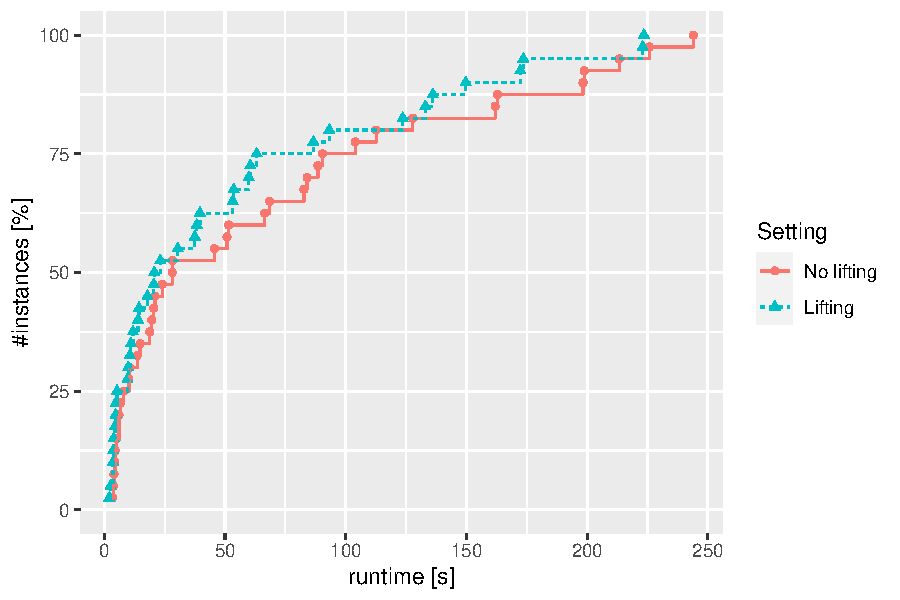
\includegraphics[width=\linewidth]{images/prepro_pmed.pdf}\label{fig:prepro_pmed}{}}
%         \end{minipage}
%         \hfill
%         \begin{minipage}[c]{.48\linewidth}
%             \subfloat[Preprocessing TSPLIB]{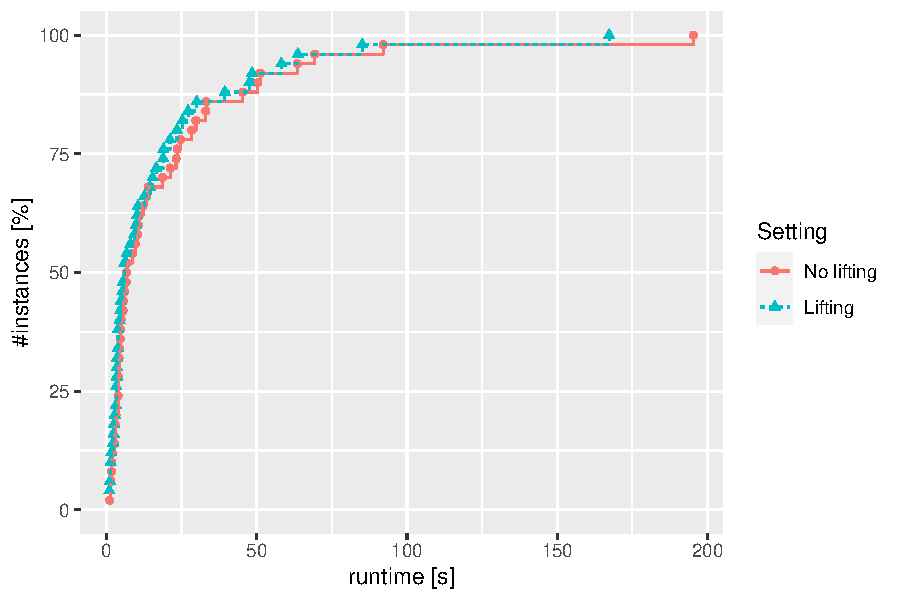
\includegraphics[width=\linewidth]{images/prepro_tsp.pdf}\label{fig:prepro_tsp}{}}
%         \end{minipage}
%         \caption{Preprocessing}\label{fig:prepro}
%     \end{figure}
% \end{frame}

% \begin{frame}{\nPC-results}
%     \begin{figure}
%         \begin{minipage}[c]{.48\linewidth}
%             \subfloat[\nPC\ optimality gap]{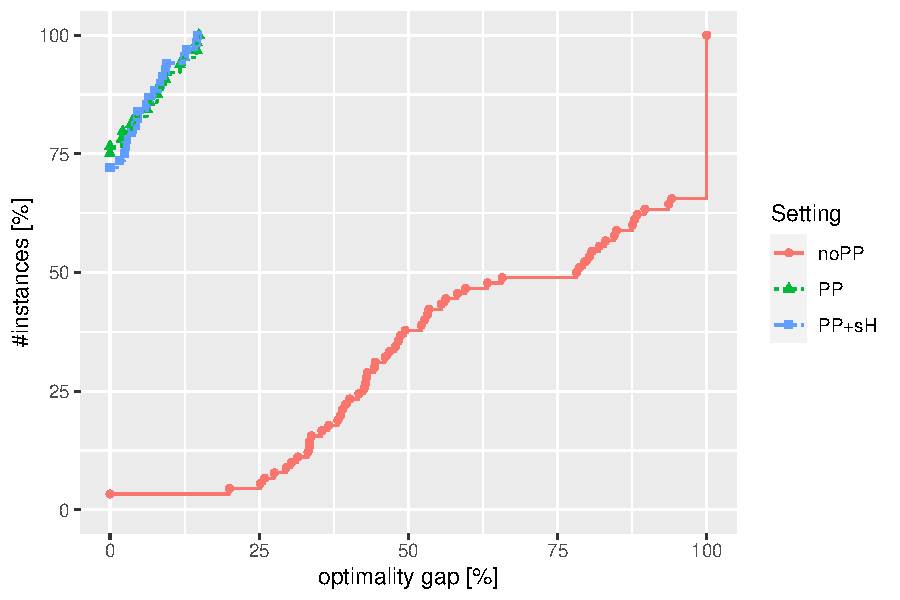
\includegraphics[width=\linewidth]{images/gap_xy_both.pdf}\label{fig:xy_gap}{}}
%         \end{minipage}
%         \hfill
%         \begin{minipage}[c]{.48\linewidth}
%             \subfloat[\nPC\ runtime]{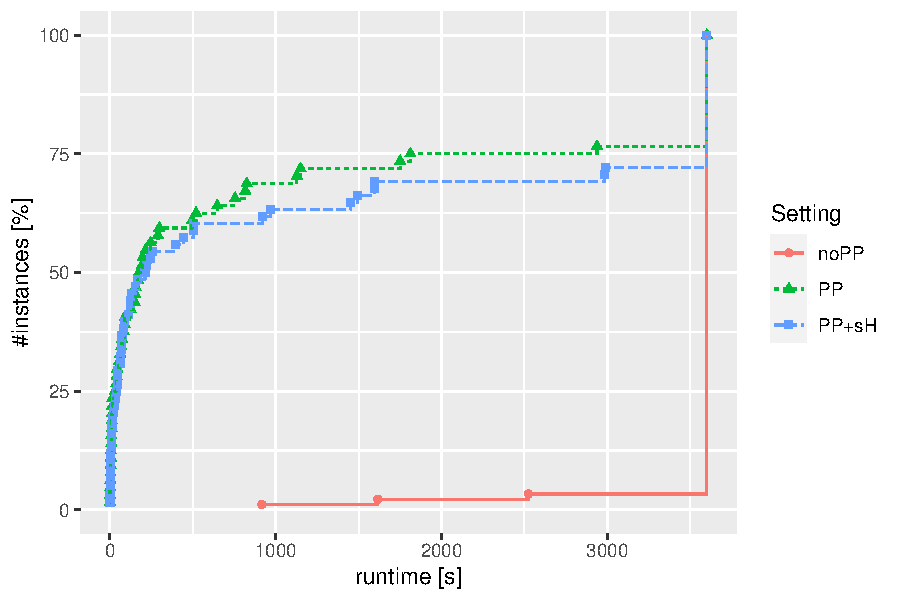
\includegraphics[width=\linewidth]{images/runtime_xy_both.pdf}\label{fig:xy_runtime}{}}
%         \end{minipage}
%         \label{fig:xy}
%         %\caption{Results of \nPC}
%     \end{figure}
% \end{frame}

% \begin{frame}{\nPCY-results}
%     \begin{figure}
%         \begin{minipage}[c]{.48\linewidth}
%             \subfloat[\nPCY\ optimality gap]{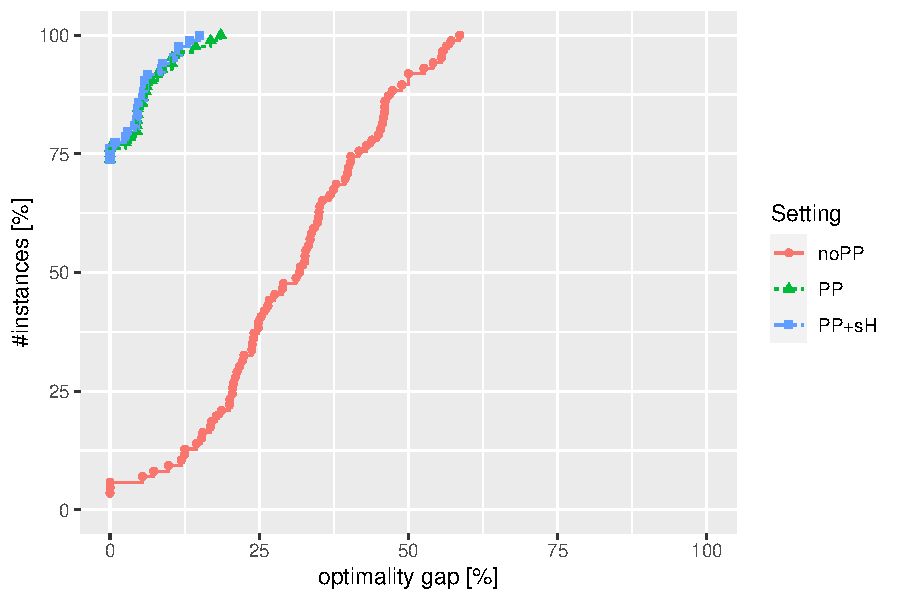
\includegraphics[width=\linewidth]{images/gap_y_both.pdf}\label{fig:y_gap}{}}
%         \end{minipage}
%         \hfill
%         \begin{minipage}[c]{.48\linewidth}
%             \subfloat[\nPCY\ runtime]{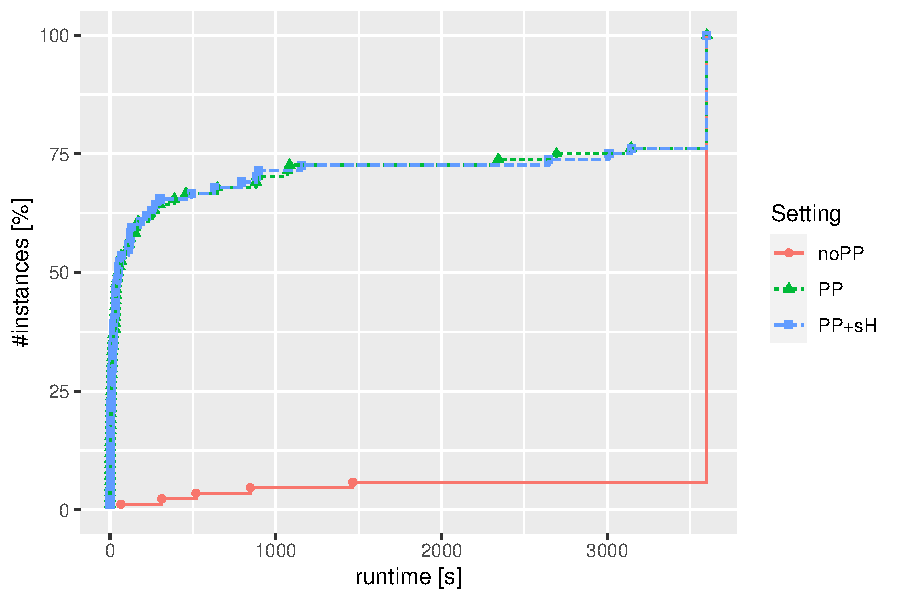
\includegraphics[width=\linewidth]{images/runtime_y_both.pdf}\label{fig:y_runtime}{}}
%         \end{minipage}
%         \label{fig:y}
%         %\caption{Results of \nPCY}
%     \end{figure}
% \end{frame}

% \begin{frame}{\nPCE-results}
%     \begin{figure}
%         \begin{minipage}[c]{.48\linewidth}
%             \subfloat[\nPCE\ optimality gap]{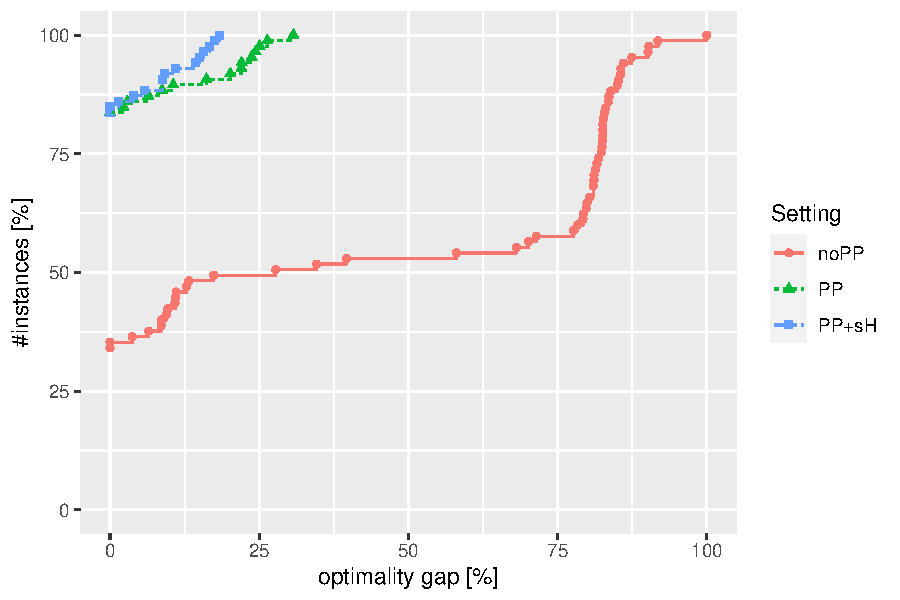
\includegraphics[width=\linewidth]{images/gap_u_both.pdf}\label{fig:u_gap}{}}
%         \end{minipage}
%         \hfill
%         \begin{minipage}[c]{.48\linewidth}
%             \subfloat[\nPCE\ runtime]{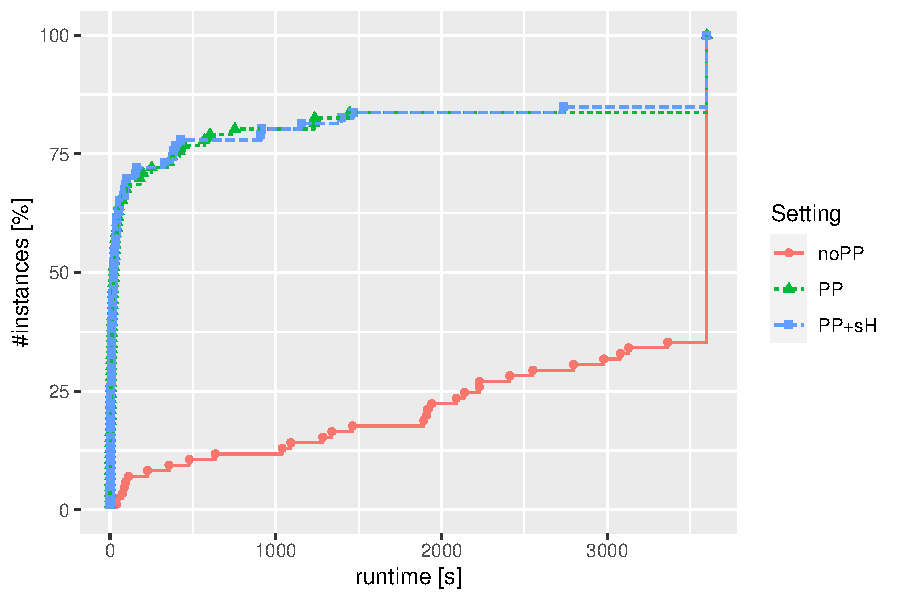
\includegraphics[width=\linewidth]{images/runtime_u_both.pdf}\label{fig:u_runtime}{}}
%         \end{minipage}
%         \label{fig:u}
%         %\caption{Results of \nPC}\label{fig:x}
%     \end{figure}
% \end{frame}

\begin{frame}{Setting comparison on formulation \nPCY}
    \begin{figure}
        \begin{minipage}[c]{.48\linewidth}
            \subfloat[Runtimes]{\includegraphics[width=\linewidth]{inoc_runtime_nPCY.pdf}\label{fig:nPC2_runtime}{}}
        \end{minipage}
        \hfill
        \begin{minipage}[c]{.48\linewidth}
            \subfloat[Optimality gaps \text{$\left[\frac{UB-LB}{UB}100\right]$}]{\includegraphics[width=\linewidth]{inoc_gap_nPCY.pdf}\label{fig:nPC2_gap}{}}
        \end{minipage}
        \label{fig:nPC2}
        %\caption{Results of \nPC}\label{fig:x}
    \end{figure}
\end{frame}

\begin{frame}{Setting comparison on formulation \nPCE}
    \begin{figure}
        \begin{minipage}[c]{.48\linewidth}
            \subfloat[Runtimes]{\includegraphics[width=\linewidth]{inoc_runtime_nPCE.pdf}\label{fig:nPC3_runtime}{}}
        \end{minipage}
        \hfill
        \begin{minipage}[c]{.48\linewidth}
            \subfloat[Optimality gaps \text{$\left[\frac{UB-LB}{UB}100\right]$}]{\includegraphics[width=\linewidth]{inoc_gap_nPCE.pdf}\label{fig:nPC3_gap}{}}
        \end{minipage}
        \label{fig:nPC3}
        %\caption{Results of \nPC}\label{fig:x}
    \end{figure}
\end{frame}


\begin{frame}{Formulation comparison on setting \sH}
    \begin{figure}
        \begin{minipage}[c]{.48\linewidth}
            \subfloat[Runtimes]{\includegraphics[width=\linewidth]{inoc_runtime_PH.pdf}\label{fig:PH_runtime}{}}
        \end{minipage}
        \hfill
        \begin{minipage}[c]{.48\linewidth}
            \subfloat[Optimality gaps \text{$\left[\frac{UB-LB}{UB}100\right]$}]{\includegraphics[width=\linewidth]{inoc_gap_PH.pdf}\label{fig:PH_gap}{}}
        \end{minipage}
        \label{fig:PH}
        %\caption{Results of \nPC}\label{fig:x}
    \end{figure}
\end{frame}

\begin{frame}{Managerial insights}
    \begin{figure}
        \begin{minipage}[r]{.48\linewidth}
            \subfloat[Relative regrets of the optimal solution value]{\includegraphics[width=\linewidth]{regret_obj.pdf}\label{fig:rel_regret}{}}
        \end{minipage}
        \hfill\pause
        \begin{minipage}[l]{.48\linewidth}
            \subfloat[Relative regrets of \# of opened facilities]{\includegraphics[width=\linewidth]{regret_fac.pdf}\label{fig:rel_fac}{}}
        \end{minipage}
        \label{fig:manage}
        %\caption{On a subset of instances: Only if the problem was solved to optimality}
    \end{figure}
\end{frame}


\begin{frame}{Conclusion}
    \begin{itemize}
        \item introduced nested $p$-center problem
        \item three mixed integer formulations
        \item improvement of formulations
        \item preprocessing brings a large speed up on all formulations
        \item starting heuristic little effect, shows good upper bound obtained in preprocessing
        \item nested facility location with uncertainty interesting for future work
        \item or nested maximum coverage problem
    \end{itemize}
\end{frame}

% \begin{frame}{Comparison}
%     \begin{itemize}
%     \setlength\itemsep{1em}
%         \item comparing the results between \nPC\ and \nPCY\ and \nPCE\ \pause
%         \item comparing the different lifting methods  \pause
%         \item analyzing the solutions of the nested and comparing it to the standard $p$-center problem \pause
%         \item analyzing the results regarding managerial insights
%     \end{itemize}
% \end{frame}

\maketitle

\section*{End of presentation}

% \begin{frame}{Formulations with non optimal instances}
%     \centering
%     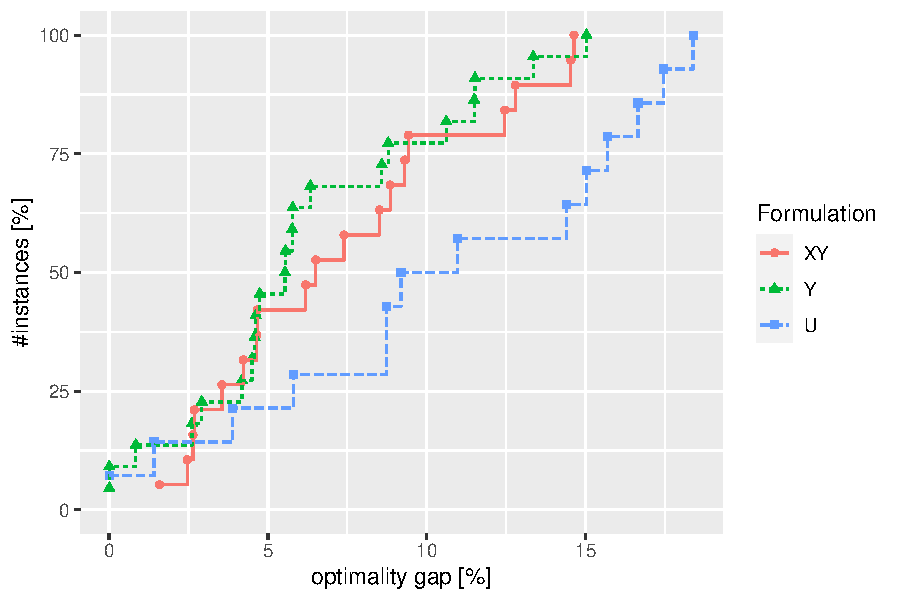
\includegraphics[width = .65\linewidth, keepaspectratio]{images/gap_models_sH_nopt.pdf}
% \end{frame}

\begin{frame}[allowframebreaks]{References}
    %\setbeamerfont{bibliography item}{size={\footnotesize}}
    %\AtNextBibliography{\footnotesize}
    \printbibliography
\end{frame}

\begin{frame}{Setting comparison on formulation \nPC}
    \begin{figure}
        \begin{minipage}[c]{.48\linewidth}
            \subfloat[Runtimes]{\includegraphics[width=\linewidth]{inoc_runtime_nPC.pdf}\label{fig:nPC1_runtime}{}}
        \end{minipage}
        \hfill
        \begin{minipage}[c]{.48\linewidth}
            \subfloat[Optimality gaps \text{$[\frac{UB-LB}{UB}]$}]{\includegraphics[width=\linewidth]{inoc_gap_nPC.pdf}\label{fig:nPC1_gap}{}}
        \end{minipage}
        \label{fig:nPC1}
        %\caption{Results of \nPC}\label{fig:x}
    \end{figure}
\end{frame}

\begin{frame}{Formulation \nPC}
    \vspace*{-23pt}
    \begin{minipage}[t]{0.48\textwidth}
        %\vspace{25pt}
        \setbeamerfont{block body}{size=\footnotesize}
        \begin{block}<1->{Decision variables}
            \vspace*{-8pt}
            \begin{alignat*}{2}
                \onslide<1->{
                 & x_{ij}^h \ldots \begin{cases}
                                           1 \, \dots \,   \text{if \emph{location \textit{i}} is \emph{assigned} to }        \\
                                           \qquad \; \,    \text{\emph{location \textit{j}} in \emph{time period \textit{h}}} \\
                                           0 \, \dots \,   \text{otherwise}
                                       \end{cases}                                                                             \\}
                \onslide<2->{
                 & y_{j}^h \ldots \begin{cases}
                                          1 \, \dots \, \text{if \emph{location \textit{j}} is \emph{open} in} \\
                                          \qquad \; \,  \text{\emph{time period \textit{h}}}                   \\
                                          0 \, \dots \, \text{otherwise}
                                      \end{cases}                                                               \\}
                \onslide<3->{
                 & z^h  \ldots  \,  \text{maximum \emph{distance} between any }                                                                      \\
                 & \qquad \; \; \,  \text{\emph{customer \textit{i}} and its nearest \emph{open facility}}                                           \\
                 & \qquad \; \; \,  \text{in period \textit{h}}}
            \end{alignat*}
            \vspace{10pt}
        \end{block}
    \end{minipage}
    \begin{minipage}[t]{0.48\textwidth}
        %\setbeamerfont{block title}{size=\small}
        \setbeamerfont{block body}{size=\footnotesize}
        \begin{block}<4->{\nPC\ based on \citet{wiley2013}}
            \vspace*{-12pt}
            \begin{subequations}
                \begin{alignat}{3}
                     & \min         & \sum_{\inH}z^{h}             &                                                                              \\
                     & \text{ s.t.} & \sum_{j \in V}y_{j}^h        & =     p^{h}           &  & \forall \inH                                      \\
                     &              & \sum_{j \in V}x_{ij}^h       & =     1               &  & \forall i \in V, \inH                             \\
                     &              & x_{ij}^h                     & \leq  y_j^{h}         &  & \forall i,j \in V, \inH                           \\
                     &              & \sum_{j \in V}d_{ij}x_{ij}^h & \leq  z^{h}           &  & \forall i \in V, \inH                             \\
                     &              & y_{j}^h                      & \geq  y_j^{h-1}       &  & \forall \inH \setminus \left \{1 \right \}        \\
                     &              & (x,y,z)                      & \in |V|^2|\mathcal H| &  & \times |V||\mathcal H| \times \mathbb{R}_{\geq 0}
                \end{alignat}  \label{eq:nPC}
            \end{subequations}
        \end{block}
    \end{minipage}
\end{frame}

\end{document}
\endinput